\chapter{Reconhecimento facial}
\label{cp:3_rec_facial}

A face é a modalidade biométrica mais utilizada, visto que apresenta severas vantagens perante as outras modalidades, por apresentar características naturais, método de coleta não intrusivo e fácil manipulação. Segundo \citeonline{lone2011automatic} essa modalidade de reconhecimento está aumentando gradativamente seu prestígio frente a segurança pessoal nas últimas décadas, conseguindo obter resultados consideráveis de confiança. Com todas essas vantagens essa modalidade biométrica vem possibilitando avanços em pesquisas biométricas com iniciativas que visam aumento de sua credibilidade e precisão no reconhecimento de pessoas.

Desde o advento da fotografia, inúmeros órgãos públicos e privados têm mantido bancos de dados de fotografias de pessoas contendo a face (por exemplo, para identificação pessoal, passaportes, cartões de associação, controle de acesso a computadores ou equipamentos, autenticação bancária, operações financeiras e utilização nos sistemas de vigilância). O interesse pelo reconhecimento automático de face está em alta devido as suas inúmeras aplicações no cotidiano, incluindo o controle de acesso e sistemas de segurança \cite{buciu2014challenges}. 


O problema de reconhecimento facial a partir de uma ou mais imagens de faces foi abordado na década de 60 por pesquisadores de visão computacional. Desde então pesquisadores têm apresentado interesse e motivações de desenvolvimento de sistemas que possibilitem maior confiabilidade em aplicações de mundo real. Conforme \citeonline{lumini2017overview} por meio da face podemos realizar análises das características faciais e identificar momentaneamente as pessoas, seu estado emocional e sua expressão facial. O reconhecimento biométrico da face é realizado a partir de técnicas de processamento de imagens da face do indivíduo capturadas por uma ou mais câmeras. 

A tarefa de reconhecimento pode ser considerada uma atividade simples quando falamos em reconhecimento por um humano.  Como sabemos o cérebro humano pode identificar corretamente uma pessoa a partir de sua imagem facial, mesmo sob as mais variadas condições do ambiente, como variações de iluminação, pose, oclusão e expressão facial, observando apenas uma de suas características ou partes dessas, e até mesmo com distorções ou deformações. Entretanto, essa atividade apresenta-se extremamente complexa ao ser implementada em um computador. Um sistema de reconhecimento facial é considerado adequado quando detecta de forma automática uma face presente na imagem adquirida e identifica a face mediante qualquer ponto de vista, independente da variação de pose, iluminação, etc.

É possível visualizar na figura \ref{fig:processo_rec} o processo necessário para identificação de uma face sem oclusão e uma face ocluída parcialmente. De maneira que podemos perceber a adição de mais quatro fases no processo de reconhecimento tradicional, adicionando um pouco mais de complexidade ao problema.


\begin{figure}[H]
\centering
\caption{Etapas necessárias para o reconhecimento de uma face sem oclusão e uma face com oclusão}
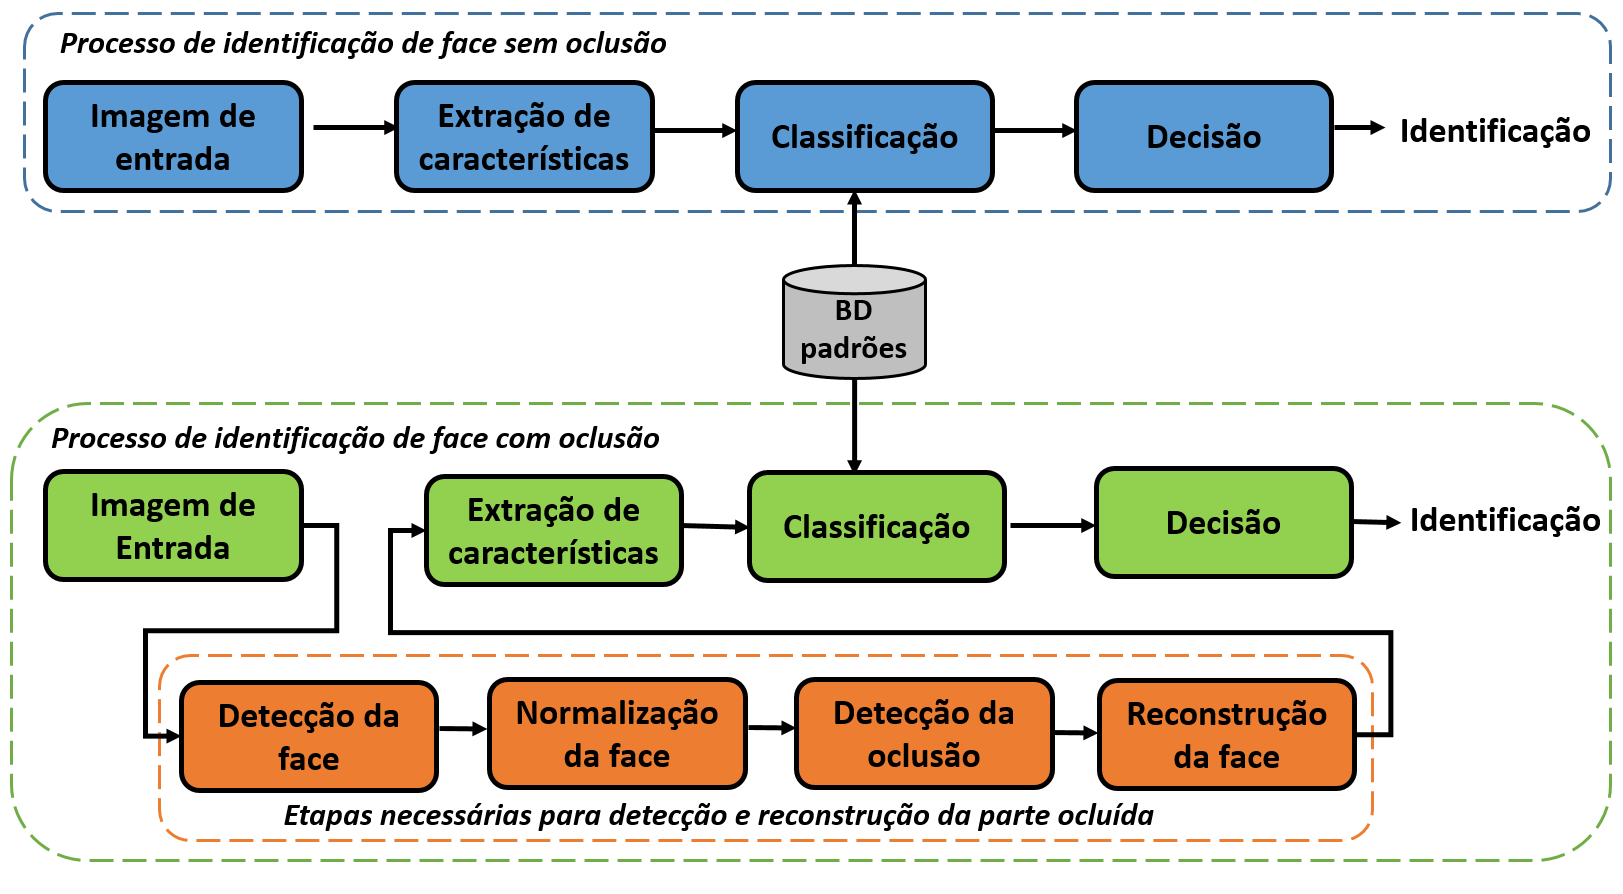
\includegraphics[scale = 0.37]{imgs3/etapas_biometricas}
\source{Jonas Mendonça Targino, 2018}
\label{fig:processo_rec}
\end{figure}



As principais abordagens que visam o reconhecimento facial são baseadas na localização e forma dos atributos faciais também conhecidos como pontos-chave, e são os olhos, sobrancelhas, nariz, boca e queixo, e suas relações espaciais tomam por base uma análise global da imagem do rosto como uma combinação de outras faces daquele mesmo rosto. Após a localização da face algumas características são extraídas da mesma analisando sua geometria facial, dentre estas características temos a análise da distância entre os pontos-chave, tais como distância entre boca e nariz, olho e nariz, queixo e olhos, etc. 



Perante a modalidade biométrica de reconhecimento de face muitas aplicações que usam tal método de segurança têm sido utilizadas, dentre as aplicações temos:

\begin{itemize}
\item sistemas de vigilância;
\item monitoramento fechado de circuito televisionado;
\item investigações de imagens;
\item reconstrução de imagens;
\item identificação de criminosos;
\item autorização de acesso.
\end{itemize}

A face como as outras modalidades biométricas possui suas vantagens e desvantagens, sendo elas:

\noindent \textbf{Vantagens:}
\begin{itemize}
\item nenhuma necessidade de contato;
\item sensores comumente usados e disponíveis (câmeras de segurança);
\item grandes quantidades de dados existentes, permitindo avaliação a partir de imagens armazenadas em \textit{backup};
\item facilidade de manipulação por humanos.
\end{itemize}


\noindent \textbf{Desvantagens:}
\begin{itemize}
\item a face pode ser obstruída por oclusões, como também outras variações (iluminação, expressão e pose);
\item mudança da face de acordo com o tempo;
\item possibilidade de fornecimento de imagens faciais de baixa resolução.
\end{itemize}


\section{Reconhecimento facial em ambientes não controlados}
A face é a modalidade biométrica  com menor grau de intrusão mediante a privacidade dos indivíduos, possibilitando comodidade e bem-estar por parte dos usuários durante o processo de coleta dos dados.  O número de sistemas de reconhecimento biométrico que usam a face como modalidade biométrica é relativamente elevado \cite{buciu2014challenges}, entretanto, o desempenho desses sistemas é apenas razoável. Esta afirmativa deve-se ao fato de que essas estratégias biométricas apresentam grandes dificuldades para manipular imagens de face coletadas em ambientes não controlados. Essas dificuldades para manipular imagens de face coletadas em ambientes não colaborativos, se dão devido as condições do ambiente e a não cooperação por parte do usuário para a coleta dos dados, essa é uma das vantagens dos ambientes não controlados.

Com o auxílio da figura \ref{fig:variacoes} podemos visualizar os tipos de variações encontradas ao lidarmos com ambientes não controlados.
 
\begin{figure}[H]
\centering
\caption{Tipos de variações advindas dos ambientes não controlados}
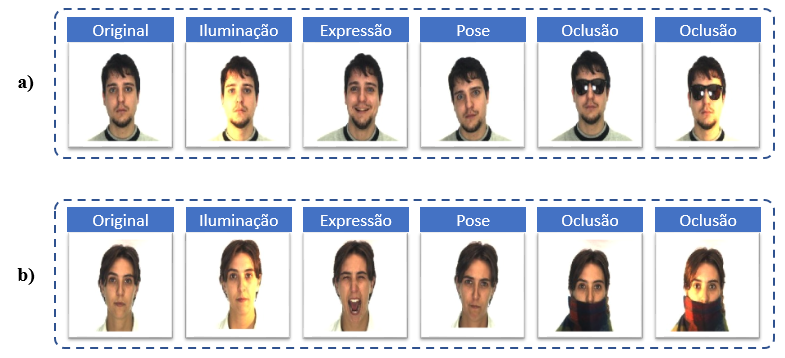
\includegraphics[scale = 0.76]{imgs/variacoes.png}
\source{Jonas Mendonça Targino, 2018. Imagens de faces obtidas da base AR \cite{martinez1998ar}}
\label{fig:variacoes}
\end{figure}

 
As imagens de face coletadas sobre condições não controladas apresentam fortes variações, estas são provindas do ambiente de coleta. A partir dessas variações surge uma lacuna na área de reconhecimento biométrico de face, dado que manipular essas variações exige-se um grande número de técnicas para detecção da face, detecção da oclusão, reconstrução da imagem da face e por fim identificação do indivíduo.
Atualmente, há progresso significativo em reconhecimento automático de faces em condições controladas. Entretanto, segundo \citeonline{[5]aisha2014face}, \citeonline{min2014efficient} e \citeonline{zhang2018fast} não pode-se afirmar o mesmo da performance quando lidamos com condições não controladas, visto que as variações presentes nestes ambientes degradam a taxa de reconhecimento.

É possível perceber com o auxílio da figura \ref{fig:variacoesAparencia} como as variações anteriormente apresentadas distanciam as imagens de mesma classe no espaço. Nessa figura são apresentados três eixos exemplificando como as variações presentes na imagem podem deslocar a imagem de um mesmo indivíduo no plano cartesiano, favorecendo com isso baixa performance de identificação. Na figura \ref{fig:variacoesAparencia} é possível perceber que a variação de iluminação favorece ao erro de reconhecimento, aproximando o indivíduo 1 do indivíduo 7. Paralelamente, com a oclusão de cachecol favorecendo o erro de reconhecimento do indivíduo 1 com o indivíduo 3.


\begin{figure}[H]
\centering
\caption{Exemplos de variações intraclasse, as quais distanciam as variações de aparência das imagens do indivíduo 1.}
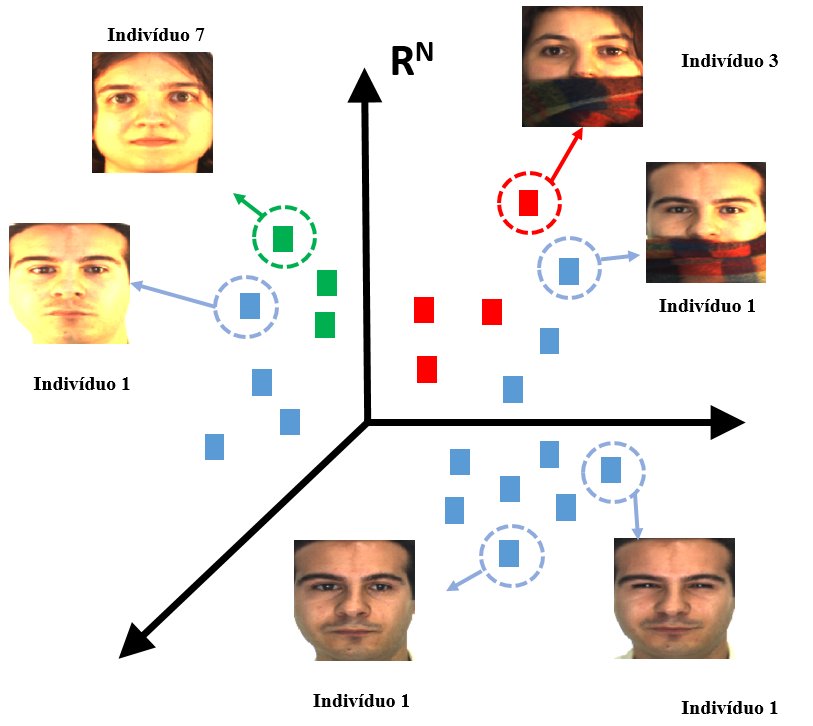
\includegraphics[scale = 0.50]{imgs/xyz2}
\source{Jonas Mendonça Targino, 2018. Imagens de faces obtidas da base AR \cite{martinez1998ar}}
\label{fig:variacoesAparencia}
\end{figure}



\section{Detecção da face}
\label{sec:detecção face}

Detecção de face é uma técnica de processamento de imagem e visão computacional que se dedica a analisar a existência ou não de uma face sobre determinada imagem e a partir disso retornar a localização espacial da mesma sobre a imagem.


Umas das atividades que devem ser realizadas na maioria dos sistemas de reconhecimento de faces \nomenclature{SRF}{System Recognition Faces}(SRF) é a detecção da presença da face em uma determinada imagem. Todavia, detectar a face antes de detectar cada ponto chave é uma ótima estratégia, impossibilitando o retrabalho. Dado que grande parte dos algoritmos tradicionais se baseiam na identificação dos pontos-chave (olhos, nariz, boca e etc.) ou pontos fiduciais na imagem da face. Uma enorme vantagem de se detectar primeiramente a região da face em uma imagem é que após a detecção da face, a procura por pontos de referência em uma face fica restrita apenas a uma certa região da imagem, com isso reduzindo a influência de ruídos no processo de identificação.


A face é completamente um objeto 3D, que recebe iluminação de inúmeras fontes de iluminação a partir de incontáveis direções. A tarefa de detecção de faces é considerada trivial para seres humanos, por ser uma atividade natural, entretanto ao tentarmos reproduzir tal problemática em computadores ficamos sujeitos a inúmeros problemas.  Segundo \citeonline{benezeth2010vision} alguns destes problemas são variações de pose, expressão, iluminação e oclusões parciais, com isso dificultando a detecção automática da face. 

A maioria das técnicas de reconhecimento facial assumem que as faces podem ser alinhadas e devidamente normalizadas (ambos geometricamente e fotometricamente). De modo que o alinhamento é tipicamente baseado na localização dos dois olhos na face. O esquema de detecção de face desenvolvido por \cite{viola2004robust} é considerado um marco, por possibilitar que faces possam serem detectadas em tempo real, mesmo na presença dos mais diversos fundos.  


\subsection{Viola-Jones}


De maneira a possibilitar menores percentuais de influência do ambiente perante a tarefa de identificação proposta pelos sistemas biométricos baseados em faces, algumas abordagens vêm sendo propostas na literatura com vistas a segmentar a região da face dentro de uma imagem. 

Uma dessas estratégias é o algoritmo Viola-Jones \cite{viola2004robust}. Essa estratégia sendo responsável por detectar faces dentro de uma imagem por meio de um processo que consiste em transformar uma imagem de entrada em uma imagem integral. De maneira que cada pixel da imagem da nova imagem representa a soma de todos a sua esquerda e acima, sendo definida por meio da equação \ref{eq:viola_1}.

\begin{equation}
\label{eq:viola_1}
I_{integral}(x,y) = \sum_{x'\leq x,y' \leq y} I(x',y') 
\end{equation}


Na equação \ref{eq:viola_1}, $I_{integral}(x,y)$ representa um pixel da imagem integral, já $I(x',y')$ representa um pixel da imagem de entrada (ou seja, a imagem original). Um exemplo desse processo pode ser visualizado na figura \ref{fig:viola8}

\begin{figure}[H]
\centering
\caption{Exemplo de construção de uma imagem integral. verde = 2, amarelo = 2+3, laranja = 2 + 4, e azul = 2+3+4+5}
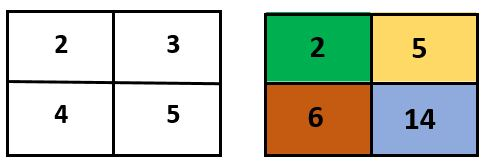
\includegraphics[scale = 0.90]{imgs/viola.png}
\source{Jonas Mendonça Targino, 2018}
\label{fig:viola8}
\end{figure}


Após a imagem integral formada torna-se possível realizar a soma de todos os pixels dentro de um retângulo apenas utilizando a soma de quatro valores. Sendo possível realizar o cálculo da soma de todos os pixels dentro de qualquer retângulo usando somente quatro valores. Sendo possível realizar a descoberta do valor de qualquer pixel do quadrado \textit{D} na imagem original, com o auxílio da equação \ref{eq:viola_2}. A descoberta do pixel \textit{D} está representado na figura \ref{fig:violaret}.


\begin{figure}[H]
\centering
\caption{Cálculo da soma de um retângulo}
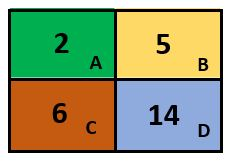
\includegraphics[scale = 0.90]{imgs/viola2.png}
\source{Jonas Mendonça Targino, 2018}
\label{fig:violaret}
\end{figure}

\begin{equation}
\label{eq:viola_2}
I(D) = D - B - C + A
\end{equation}

Tomando por base que o retângulo \textit{A} está presente nos retângulos \textit{B} e \textit{C}, torna-se necessário ao final adicionar o valor de A.

O algoritmo Viola-Jones utiliza como base retângulos para analisar determinada região da imagem. Podendo utilizar em cada análise dois ou mais retângulos seguindo diferentes tipos, em que cada tipo apresenta suas especificidades.

\begin{figure}[H]
\centering
\caption{Exemplos de características de Haar }
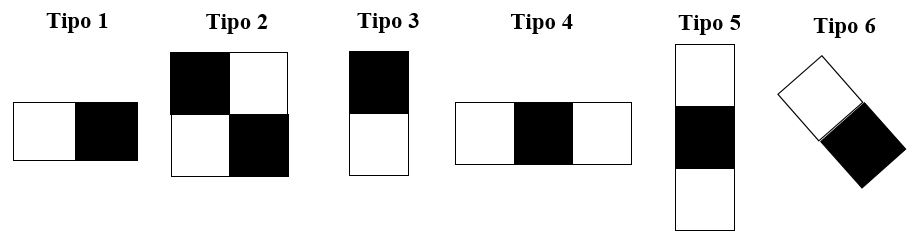
\includegraphics[scale = 0.58]{imgs/viola3.png}
\source{Jonas Mendonça Targino, 2018}
\label{fig:viola2}
\end{figure}

Esse algoritmo é muito aplicado a imagens de tamanho (24 x 24) pixels utilizando no total 6060 características de Haar diferentes. Embora o conjunto de características atuem em imagens de tamanho (24 x 24), eles possuem consideráveis resultados de eficiência computacional.

O Viola-Jones possui como estratégia varrer a mesma imagem inúmeras vezes, alternando a cada vez o tamanho de suas janelas, objetivando com isso localizar as faces presentes na imagem. A principal iniciativa do algoritmo é  gerar uma grande quantidade de janelas, analisá-las e verificar seu resultado. Ao apresentar-se resultados negativos é possível concluir que aquela região não seja uma face. Com isso, o algoritmo descarta as regiões que não são faces.

Esse algoritmo utiliza um conjunto de classificadores fracos em cascata para formar um classificador forte com consideráveis taxas de confiabilidade, seguindo uma classificação em cascata baseada na modificação do algoritmo Adaboost proposto por \citeonline{freund1999short}.

Cada nível do classificador em cascata busca analisar se naquela janela encontra-se uma face ou não. Ao identificar-se em qualquer um dos níveis que uma determinada janela é classificada como não face, aquela janela é automaticamente descartada. Entretanto, caso essa janela seja classificada como face, essa é repassada para o próximo nível da cascata. Na figura \ref{fig:viola5} pode-se visualizar o procedimento de identificação de janelas como face ou não face.

\begin{figure}[H]
\centering
\caption{Funcionamento do Viola-Jones perante o classificador em cascata }
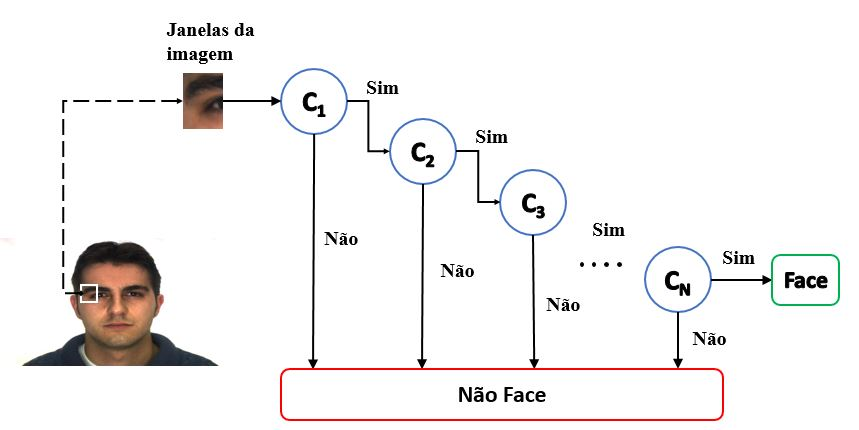
\includegraphics[scale = 0.7]{imgs/viola6.jpg}
\source{Jonas Mendonça Targino, 2018. Imagem de face obtida da base AR \cite{martinez1998ar}}
\label{fig:viola5}
\end{figure}

Uma característica importante desses classificadores é que as regiões que não são faces são descartadas logo nos primeiros níveis de classificação. 

Este algoritmo ao lidar com detecção de faces em ambientes controlados apresenta consideráveis resultados, entretanto ao lidar com ambientes não controlados essa estratégia apresenta algumas dificuldades de localização da face perante a imagem. Isso se deve variações na iluminação, expressão, pose e oclusão presentes nesses ambientes.



\subsection{Skin Tone}
\label{sub:skin}

Uma estratégia também utilizada no contexto de detecção de faces é o \textit{Skin Tone}, essa técnica proposta por \citeonline{cheddad2009skin} tem como objetivo detectar faces humanas a partir da análise da textura de cores de peles humanas. Essa técnica utiliza imagens RGB (do inglês: Red, Green, Blue) com dimensões $(d_1, d_2, 3)$, de modo que $d_1$, $d_2$ e 3 representam respectivamente a quantidade de pixels em $x$, $y$ e os canais de cores.


Para detectar os pixels de pele essa técnica utiliza alguns passos, sendo eles: 

\begin{enumerate}
\item cada pixel da imagem RGB é multiplicado pelos escalares (0.298, 0.587 e 0.140 respectivamente) e somados, gerando assim uma imagem bidimensional em escala de cinza \textit{I} de dimensões($d_1,d_2$). Conforme afirma \citeonline{cheddad2009skin} esses limiares dessa técnica foram tomados de acordo com o grau de percepção do espectro visual humano;
 
\item na segunda etapa é gerada a imagem $\hat{I}$ de dimensões ($d_1,d_2$), obtida por meio valor máximo dos pixels dos canais G e B da imagem de consulta. Os valores do canal R são ignorados, visto que a maior parte das cores de pele se apresentam de forma mais significativa nesse canal. A equação \ref{eq:skin_max} apresenta tal processo;

\item Enquanto na terceira etapa  é realizado o cálculo do erro de sinal, de modo que esse erro é proveniente da equação \ref{eq:skin_erro}.

\item Na última etapa, é gerada a imagem binária a partir da análise de limiar, esse limiar sendo disposto na literatura segundo \citeonline{cheddad2009skin} como segue a equação \ref{eq:skin_binario} para geração da imagem binária.
  
\end{enumerate}



\begin{equation}
\label{eq:skin_max}
\hat{I} = max (G(i,j), B(i,j))
\end{equation}



\begin{equation}
\label{eq:skin_erro}
E = I - \hat{I}
\end{equation}

\begin{equation}
\label{eq:skin_binario}
I_{Binaria} = \left\{\begin{matrix}
1 & se & 0.02511 \leq E(x,y) \leq 0.1177 \\ 
0 &
\end{matrix}\right.
\end{equation}



%É possível perceber no algoritmo \ref{alg:algoritmo_skin} como é o processo de detecção da face por meio da estratégia Skin Tone
%
%
%\begin{algorithm}[H]
%\caption{Skin Tone}
%\label{alg:algoritmo_skin}
%\begin{algorithmic}[1]
%
%%\Procedure{Skin Color}{}
%\State $im \gets imagem$
%\State $[w,h,a] \gets dimensoes(im)$
%%\for{i \gets 0 : 1}
%%\State $bw = zeros(l,c)$
%\For{$i = 1$ to $w$}
%	\For{$j = 1$ to $h$}
%      \State $I(w,h) \gets im(w,h,1)*0.298 + im(w,h,2)*0.587 + im(w,h,3)*0.140$
%     
%	\EndFor
%\EndFor
%
%\For{$i = 1$ to $w$}
%	\For{$j = 1$ to $h$}
%      \State $\hat{I}(w,h) = max( im (w,h,2), im(w,h,3))  $ 
%     \EndFor
%\EndFor
%\State $E = I - \hat{I}$
%     
%\For{$i = 1$ to $w$}
%	\For{$j = 1$ to $h$}
%     
%     \If {$E(w,h) <= 0.0251$  \&  $E(w,h) >= 0.1177$ }
%            \State $Face(w,h) = 1$
%      \Else
%      		\State $Face(w,h) = 0$
%             
%    \EndIf
%      
%	\EndFor
%\EndFor
%\State $retorne Face$
%
%%\EndProcedure
%\end{algorithmic}
%\source{Cheddad et al (2009)}
%\end{algorithm}

A figura \ref{fig:skincolor} ilustra a aplicação da técnica \textit{Skin Tone} em imagens de face de um mesmo indivíduo com variações de iluminação, pose e oclusão. Nessa mesma figura podemos perceber que a técnica não se sobressai bem quando apresentada a imagens de face com variações de iluminação.

\begin{figure}[H]
\centering
\caption{Exemplos de faces após a aplicação da técnica \textit{Skin Tone}}
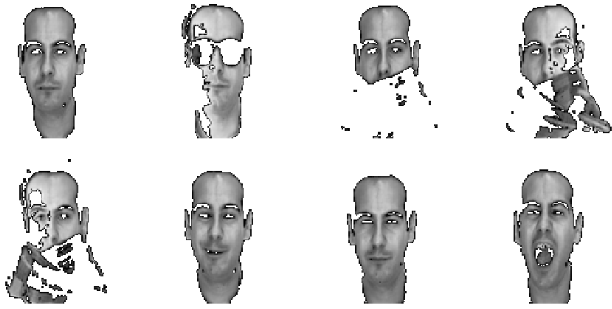
\includegraphics[scale = 0.70]{imgs/skin.png}
\source{Jonas Mendonça Targino, 2018}
\label{fig:skincolor}
\end{figure}


 

\section{Detecção de oclusão}
\label{sec:det.occlusão}
Oclusão é o posicionamento de algo, a frente do que desejamos visualizar, impedindo uma visão holística do que está por trás. Trazendo para o contexto de reconhecimento facial, \citeonline{chandel2015occlusion} afirmam que a oclusão é o elemento básico que limita a informação da imagem. Segundo \citeonline{ragashe2015approach} existem dois tipos de oclusão, a primeira é a oclusão natural, esta refere-se a obstrução da visão sem nenhuma intencionalidade, como cicatrizes e pinturas ao considerarmos o contexto de face. O segundo tipo é a oclusão artificial, esta é o foco principal deste trabalho, e a mesma se refere ao bloqueio artificial ou intencional de cobertura da imagem facial; alguns objetos como óculos, lenços, mãos e cabelos são responsáveis por gerar esse tipo de oclusão. 

A oclusão de óculos é o tipo mais comum de oclusão que afeta significativamente a performance dos sistemas de reconhecimento \cite{park2005glasses}.  Segundo \citeonline{venkatakrishnan20143d}, quando lidamos com sistemas de natureza não controlada a presença de oclusões é considerada frequente. Dessa forma, a oclusão parcial altera a aparência da face, causando reduções de desempenho do sistema, mas também levando a sérios problemas de segurança \cite{oloyede2017evaluating}.

Quando estamos diante de uma face com oclusão temos que lidar com algumas estratégias algorítmicas como forma de reparação e reconstrução da face para logo em seguida realizar a identificação frente o sistema de reconhecimento. De acordo com \citeonline{[4]wei2014dynamic} faces são facilmente ocluídas em cenários reais, alguns exemplos são objetos na frente da face (telefones celulares, alimentos e mãos), sendo muito comum diariamente  as pessoas usarem acessórios faciais, tais como, óculos de sol, lenços, chapéus, cachecóis, máscaras e véus por motivos pessoais, culturais ou até mesmo estéticos. Esses fatores são oclusões e eles podem destruir a informação discriminante  essencial da região facial, direcionando a estratégia de reconhecimento facial rumo a insuficiência de dados faciais, e com isso consequentemente dirigindo-a para uma classificação incorreta, especialmente quando a oclusão ocupa regiões consideráveis da face. 
 \citeonline{srinivasan2014occlusion} e \citeonline{tan2009face} relatam a variabilidade de condições e suas respectivas dificuldades ao se trabalhar com ambientes de coleta de imagens de face em ambientes não colaborativos com faces parcialmente ocluídas.

Lidar com oclusões parciais em imagens de face é uma tarefa complexa, pois além de identificarmos a face, temos que normalizá-la,  segmentar a mesma, aplicar algumas transformações e tentar identificar a região que a oclusão ocupa sobre a face, extrair suas características, remover essa oclusão e tentar reconstruir a face de acordo com as características que foram extraídas. Estes passos atribuem complexidade a tarefa de reconhecimento de faces em ambientes irrestritos, sem contar que as oclusões parciais possibilitam localizações errôneas das características faciais. A oclusão parcial da face é um dos problemas mais desafiadores no reconhecimento facial \cite{ekenel2009facial}. A figura \ref{fig:imgsOcluidas} apresenta algumas imagens faciais parcialmente ocluídas.

\begin{figure}[H]
\centering
\caption{Exemplos de imagens faciais ocluídas provenientes da base AR}
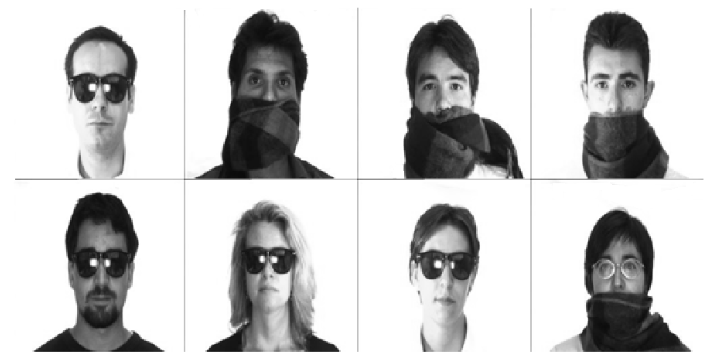
\includegraphics[scale = 0.8]{imgs/imgsOcluidas.png}
\source{Jonas Mendonça Targino, 2018. Imagens de faces obtidas da base AR \cite{martinez1998ar}}
\label{fig:imgsOcluidas}
\end{figure}

\section{Reconstrução da face ocluída}
\label{sec: reconst. face}
A reconstrução da face é uma das tarefas mais importantes perante o cenário de identificação de uma pessoa. Essa estratégia é o processo de reconstruir a imagem da face de um indivíduo (cuja identidade muitas vezes não é conhecida).


Um dos desafios das técnicas para as técnicas de reconstrução de faces é a oclusão, pois a tarefa de reconstrução exige um número considerável de imagens da face, com motivações a reconstruir tal imagem a partir da remoção da oclusão, a partir de técnicas de reconstrução de faces como, distância do vizinho mais próximo, espelhamento a partir da localização dos pontos-chave da face, dentre outras.
Um problema em reconstrução de faces é a eliminação de ruídos, esta tarefa deve ser analisada com atenção para evitar possíveis perdas de pixels considerados importantes. Por isso, algumas técnicas de reconstrução substituem apenas os pixels ocluídos pelos pixels da imagem reconstruída, fixando os pixels não ocluídos da imagem original, e com isso evitando inserção de pixels ruidosos nas posições dos pixels originais.


De acordo com   \citeonline{tajima2013performance} as técnicas de reconstrução são baseadas em subespaço e modelos. Nas abordagens baseadas em subespaço, os atributos são extraídos diretamente dos pixels da imagem da face e com isso, as imagens do conjunto são projetadas em um espaço de faces. As técnicas que seguem essa abordagem são geralmente mais fáceis de serem implementadas, entretanto, as principais desvantagens dessas técnicas é sua alta sensibilidade às condições do ambiente, como ângulo de visualização da câmera, variações de iluminação, expressão e oclusão. Enquanto, as abordagens baseadas em modelo são construídos modelos que representam o conjunto, tendo como principal vantagem a baixa sensibilidade às variações das condições do ambiente \cite{buciu2014challenges}. 



\section{Técnicas para validação das imagens reconstruídas}

Na literatura existe uma quantidade considerável de métricas que possibilitam mensurar a qualidade de duas imagens, entretanto, neste trabalho são apresentadas  três das métricas mais utilizadas. As quais são descritas com mais detalhes logo abaixo.

\subsection{Pico de Relação Sinal Ruído}

Uma das técnicas utilizadas para avaliação da qualidade da imagem reconstruída foi a Relação Sinal-ruído de pico (do inglês: \textit{Peak Signal to Noise Ratio} - PSNR) \nomenclature{PSNR}{Peak signal-to-noise ratio} proposta por \cite{ashin2005image}. Essa estratégia realiza a validação das imagens reconstruídas com imagens do respectivo indivíduo na base de treinamento. O processo de validação da imagem analisa a variação entre o valor máximo de um sinal e a potência do ruído de distorção que afeta a qualidade da imagem. 


Quanto maior o valor do PSNR, melhor é a qualidade da imagem reconstruída. A fórmula para o cálculo do PSNR é apresentada na equação \ref{eq:PSNR}.

\begin{equation}
PSNR = 10log_{10}(\frac{max^{2}}{MSE})
\label{eq:PSNR}
\end{equation}

 O cálculo do \textit{MSE} é apresentado na equação \ref{eq:MSE}, em que $I_1$ é a imagem original, $I_2$ é a imagem reconstruída e $d_1$ e $d_2$ são os números de linhas e colunas respectivamente. A métrica de análise  de qualidade da imagem reconstruída é baseada no \textit{MSE}, caso este seja maior que 30, pode-se considerar a imagem reconstruída como de boa qualidade.

\begin{equation}
MSE = \frac{\sum _{m=1}^{d_1} \sum _{n=1}^{d_2} \Big[I_1(m,n) - I_2(m,n) \Big]^2  } {d_1d_2}
\label{eq:MSE}
\end{equation}




\subsection{Similaridade Estrutural}
\label{sub:ssim}
Com forma de mensurar o quão boa foi a imagem reconstruída, nesse trabalho utilizou-se Similaridade Estrutural (do inglês: \textit{Structural Similarity} - SSIM) proposta por \cite{ssim2004}. Essa estratégia mede a similaridade entre duas imagens, neste caso a imagem reconstruída e a imagem daquele respectivo indivíduo na base de treinamento. Essa métrica produz um valor no intervalo [0,1] de modo que quanto mais próximo de 1 o valor da SSIM melhor é qualidade da imagem reconstruída. Logo o valor 1 significa as duas imagens são iguais, já se o valor é 0 significa que as duas imagens não apresentam nenhuma correlação.

A SSIM possui como base o cálculo de três fatores dada uma imagem, sendo eles: (\textit{i}) iluminação; (\textit{ii}) contraste; (\textit{iii}) estrutura da imagem. De modo que o valor da SSIM é calculado a partir de uma combinação entre esses três fatores. A SSIM pode ser obtida por meio da equação \ref{eq:SSIM}. 

\begin{equation}
\label{eq:SSIM}
SSIM(x,y)=[l(x,y)]^\alpha \cdot[c(x,y))]^\beta \cdot [s(x,y)]^\gamma
\end{equation}

De modo que $\alpha$, $\beta$ e $\gamma$ são valores que por padrão apresentam o valor 1. A iluminação nessa técnica é representada pela equação \ref{eq:ssim_iluminacao}. 

\begin{equation}
l(x,y) = \frac{2\mu_x \mu_y + C_1}{\mu_x^2 + \mu_y^2 + C1}
\label{eq:ssim_iluminacao}
\end{equation}

Já o contraste e a estrutura de uma imagem podem serem obtidos com o auxílio das equações \ref{eq:ssim_contraste} e \ref{eq:ssim_estrutura} respectivamente.

\begin{equation}
c(x,y) = \frac{2\sigma_x \sigma_y + C_2}{\sigma_x^2 + \sigma_y^2 + C2}
\label{eq:ssim_contraste}
\end{equation}



\begin{equation}
s(x,y) = \frac{\sigma_{xy} + C_3}{\sigma_x\sigma_y + C3}
\label{eq:ssim_estrutura}
\end{equation}

\begin{equation}
SSIM(x,y) = \frac{(2\mu_x\mu_y + C_1) (2\sigma_{xy} +C_2)}{(\mu_x^2 + \mu_y^2 + C1) (\sigma_x^2 + \sigma_y^2 + C_2)}
\end{equation}

Já $\mu_x$, $\mu_y$ são as médias locais de $x$ e de $y$, $\sigma_x$, $\sigma_y$ são os desvios padrão de $x$ e $y$, e por último o $\sigma_{xy}$ significa a covariância entre $x$ e $y$.


\begin{equation}
C_3 = \frac{C_2}{2}
\end{equation}

Segundo \citeonline{thung2009survey} a SSIM tenta simular o sistema visual humano por meio da análise da iluminação, contraste e estrutura da imagem fornecendo uma boa aproximação de percepção da diferença entre duas imagens.


\subsection{Erro quadrático médio}

O erro quadrático médio (do inglês: \textit{Root-mean-square error} - RMSE) \cite{chai2014root}, é uma métrica muito utilizada para analisar diferença de valores entre duas amostras. Também podendo ser utilizada para a análise da qualidade de duas imagens, a partir do erro médio quadrático dos pixels das duas imagens. O RMSE representa o desvio padrão das duas imagens, no caso a imagem modelo e a imagem comparada. Essa técnica no contexto de análise da qualidade das imagens busca verificar a magnitude dos erros existentes entre duas imagens.

A equação do RMSE pode ser obtida com o auxílio da equação \ref{eq:rmse}. Em que $I_1$ e $I_2$ são respectivamente a imagem modelo e a imagem comparada. E $P$ é o número de pixels de cada imagem. Deste modo, é possível deduzir que o RMSE quando aplicado ao contexto de análise de imagens é a raiz quadrada da média dos erros quadrados dos pixels. Assim, quanto maior o erro por pixel maior o RMSE.

\begin{equation}
RMSE = \sqrt{\frac{\sum_{p=1}^{P} (I_1 - I_2)^2 }{P}}
\label{eq:rmse}
\end{equation}

Os valores dessa métrica são sempre positivos, e um valor 0 indica que as duas imagens são semelhantes. Logo quanto menor o RMSE, melhor é a qualidade das imagens.


\section{Análise de desempenho}

Existem algumas métricas que possibilitam fazer uma análise um pouco mais detalhada de cada técnica, possibilitando inferências sobre o comportamento de cada técnica. Sem necessariamente utilizar apenas a taxa de reconhecimento como fator decisivo de julgamento que uma técnica é melhor que outra.


\subsection{Taxa de falsa aceitação e falsa rejeição}
Ao lidarmos com identificação, o modelo é treinado com várias imagens de várias pessoas, e para aquele conjunto de pessoas, um modelo biométrico é treinado de modo a identificar essas pessoas. Dessa forma para que um padrão possa ser reconhecido é necessário uma comparação de similaridade entre todos os modelos conhecidos, produzindo uma pontuação ou uma alguma medida de similaridade que possa descrever de forma numérica o quão similares é o padrão de consulta e o modelo. Logo, o sistema atribui o padrão de consulta à pessoa com maior similaridade do modelo biométrico. Visto isso, de modo a evitar possíveis impostores (pessoas não contidas no conjunto), os sistemas biométricos utilizam algumas métricas, para tentar evitar problemas como esse, de maneira que essas métricas possuem um limiar de similaridade entre a imagem de consulta e o modelo, de modo que caso esse limiar não seja alcançado o padrão de consulta é rejeitado.

Esses limiares são usados para expressar a similaridade entre um padrão de entrada e o modelo biométrico. Logo quanto maior a similaridade, maior será a semelhança entre o padrão e o modelo. Nos sistemas biométricos a pontuação obtida pela análise de similaridade entre a consulta e o modelo é fundamental para separar os grupos de indivíduos presentes na base e indivíduos impostores.

Entretanto, segundo \citeonline{costa2011ensemble} em aplicações reais em alguns casos, os padrões biométricos dos impostores possuem pontuações mais altas do que alguns padrões de clientes. Por tal motivo, ao selecionar um limiar de classificação pode implicar em erros para a tarefa de classificação. Por exemplo, a escolha de um limiar muito alto pode assegurar que nenhum impostor com pontuação tão alta excederá tal limite, possibilitando que nenhum falso positivo seja aceito pelo sistema. Consequentemente, os padrões de usuários com pontuações mais baixas do que as pontuações mais altas dos impostores serão rejeitados, implicando em uma falsa rejeição. Logo, a escolha de um bom limiar deve ser tomada com base em uma estratégia que reduza o índice de falsos reconhecimentos e falsas aceitações.

O trabalho de \citeonline{prabhakar2003biometric} apresenta duas distribuições que podem ser utilizadas para descoberta de um bom valor de limiar. Uma delas é a taxa de falsa aceitação (do inglês: \textit{False Acceptance Rate} - FAR) que é a medida de probabilidade de um sistema biométrico aceitar de maneira incorreta um indivíduo não autorizado (impostor), logo a FAR de um sistema é obtida por meio da razão envolvendo o número de falsas aceitações pela quantidade de tentativas de reconhecimento. 

E a outra é a falsa rejeição (do inglês: \textit{False Recognition Rate} - FRR) que significa o percentual de rejeições feitas incorretamente pelo sistema biométrico, de modo que o sistema falha em reconhecer uma pessoa autorizada, rejeitando essa pessoa como um impostor. Logo a FRR é declarada como número de falsas identificações dividido pelo número de falsos reconhecimentos. O ponto de cruzamento entre as curvas de FAR e FRR é chamado de igual taxa de erro (do inglês: \textit{Equal Error Rate} - ERR), logo, o ponto ERR é o limiar ótimo para o sistema, visto que nesse ponto o percentual de falsas aceitações e falsas rejeições são iguais. A figura \ref{fig:FAR_FRR_ERR} ilustra as curvas de FAR e FRR, como também o ponto de cruzamento ERR das duas curvas.


\begin{figure}[H]
\centering
\caption{Curvas de FAR, FRR e ponto de intersecção EER }
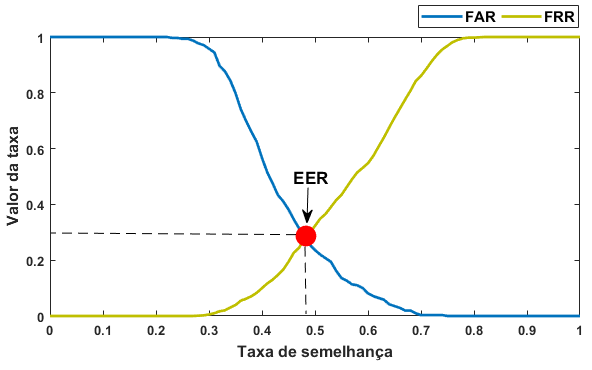
\includegraphics[scale = 0.70]{imgs4/FAR_FRR_ERR}
\source{Jonas Mendonça Targino, 2018}
\label{fig:FAR_FRR_ERR}
\end{figure}

Visto que o ERR é o limiar ótimo de aplicação de tal técnica no sistema de reconhecimento, é interessante percebermos que ao aumentar a taxa de semelhança maior que o EER maior será o número de rejeições de indivíduos cadastrados na base, e ao diminuirmos o EER maior será a aceitação de impostores pelo sistema de reconhecimento.

\subsection{Matriz de confusão}

Outra forma de mensurar o quão boa é uma determinada técnica perante a tarefa de identificação frente ao sistema é analisar a matriz de confusão. Esta, sendo responsável por fornecer uma visão geral da técnica, mostrando o número de classificações corretas, como também a classificação predita para cada classe, para um conjunto de exemplos.	


A Matriz de confusão  representa em forma matricial os rótulos de saída do classificador e a sua respectiva saída desejada para cada classe. A posição $i$ (linha) da matriz apresenta os valores esperados para cada amostra, enquanto a posição $j$ (coluna), apresenta os valores preditos pelo modelo. Dessa forma, cada posição $(i,j)$ da matriz apresenta o número de amostras da classe $i$ que foram preditas pelo modelo como sendo da classe $j$. Um fato interessante da matriz de confusão é que a quantidade presente na diagonal principal é o número de amostras que o modelo julgou corretamente, nesses pontos da diagonal $i=j$. Ou seja, o número de acertos para cada classe se localiza na diagonal principal da matriz de confusão, e os demais elementos da matriz representam erros na classificação.

Enquanto para o problema de classificação binário, no qual a saída desejada pode ser codificada como  [0,1], a matriz de confusão pode ser vista conforme a figura \ref{fig:matriz_confusao}, em que os valores de VP, FN, FP e VN, representam respectivamente,  verdadeiros positivos (amostras positivas classificadas corretamente),  falsos negativos (quantidade de amostras que foram preditas pelo modelo como sendo da classe 0, quando na verdade pertenciam a classe 1), falsos positivos (quantidade de amostras que foram preditas como sendo da classe 1, mas eram da classe 0) e  verdadeiros negativos (quantidade de amostras corretas que foram preditas pelo modelo como sendo da classe 0).

\begin{figure}[H]
\centering
\caption{Estrutura de uma matriz de confusão}
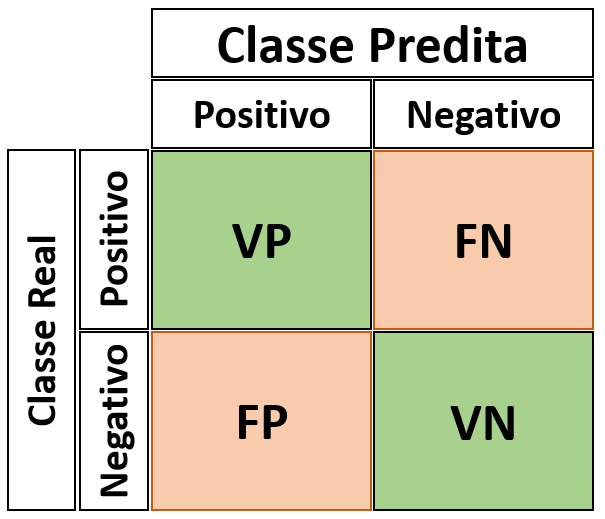
\includegraphics[scale = 0.45]{imgs4/matrix_confusion}
\source{Jonas Mendonça Targino, 2018}
\label{fig:matriz_confusao}
\end{figure}

Uma grande contribuição da matriz de confusão é a possibilidade de visualizar quais classes estão apresentando maior erro e maior acerto. Também sendo possível com essa matriz obter algumas métricas que podem nos auxiliar quanto a análise da técnica após sua classificação. Algumas dessas métricas são:

\begin{itemize}

\item \textbf{Acurácia} - Significa a taxa de acerto das classes positivas e negativas perante todas as amostras. A acurácia pode ser calculada com o auxílio da equação \ref{eq:acuracia}, em que $P$ é o número de amostras positivas e $N$ é o número de amostras negativas. 
\begin{equation}
acuracia = \frac{VP + VN}{P + N}
\label{eq:acuracia}
\end{equation}

\item \textbf{Sensibilidade} - Significa a probabilidade do classificador	identificar corretamente os indivíduos da classe positiva. A sensibilidade pode ser calculada com o auxílio da equação \ref{eq:sensibilidade}.
\begin{equation}
Sensibilidade = \frac{VP}{VP + FN} 
\label{eq:sensibilidade}
\end{equation}

\item \textbf{Especificidade} - Significa a probabilidade do classificador identificar corretamente os indivíduos da classe negativa. A equação \ref{eq:especificidade} apresenta a fórmula para o cálculo da especificidade. 
\begin{equation}
especificidade = \frac{VN}{VN + VP}
\label{eq:especificidade}
\end{equation}


\item \textbf{F1-score} - É uma métrica que utiliza como base a média ponderada entre a precisão e a sensibilidade. Podendo ser obtida com o auxílio da equação \ref{eq:fscore}. O F1-score retorna um valor no intervalo [0,1], de modo que 1 representa seu melhor valor (precisão e sensibilidade perfeitas) e 0 indica os piores resultados de precisão e sensibilidade. 

\begin{equation}
f_1score = 2 \times \frac{precisao\times sensibilidade}{precisao + sensibilidade}
\label{eq:fscore}
\end{equation}

\item \textbf{Coeficiente de correlação de de Matthews} (do inglês: \textit{Matthews correlation coefficient} - MCC) - É uma medida utilizada na área de aprendizado de máquina a qual possibilita mensurar a qualidade das duas classes na matriz de confusão. Essa métrica tem como base a estabilidade do desbalanceamento entre as classes, levando em conta os VP, FP e FN. O MCC pode ser aplicado independentemente dos tamanhos diferentes entre as classes. O MCC retorna um valor no intervalo [-1,+1], de modo que +1 representa uma predição perfeita, 0 indica que a predição é inferior a uma predição aleatória, e -1 indica discordância total entre o real e o predito. Essa métrica pode ser calculada diretamente com o auxílio da matriz de confusão com a ajuda da equação \ref{eq:mcc}.

\begin{equation}
MCC = \frac{VP \times VN - FP \times FN}{\sqrt{(VP + FP)(VP + FN)(VN + FP)(VN + FN)}}
\label{eq:mcc}
\end{equation}


\item \textbf{Curva Roc} - É um gráfico comumente utilizado que permite sumarizar a performance de uma determinada técnica a partir de vários limiares entre [0,1]. De modo que esse gráfico possui em um de seus eixos (eixo y) a taxa de verdadeiros positivos e em outro eixo (eixo x) a taxa de falsos positivos. Desse modo permitindo limiares de aplicação da técnica no mundo real. De modo que possamos enxergar limiares que condigam com as prioridades de aplicação. Em que essas prioridades possam ser definidas como percentual de falsos negativos ou falsos positivos.
\end{itemize}


\section{Considerações finais do capítulo}

Este capítulo apresentou conceitos da área relacionada com o tema desta pesquisa, permitindo conhecimento do contexto em que essa pesquisa se insere. Vindo a apresentar conceitos relacionados a biometria e sua contribuição frente a sociedade na tarefa de reconhecimento de pessoas. Como também apresentou os prós e contras de trabalharmos com ambientes não controlados, em que percebeu-se que a detecção da oclusão é a variação menos estudada pela comunidade científica. Logo apresentando o processo necessário para se trabalhar com oclusões parciais em imagens de face. Neste capítulo também foram apresentadas duas técnicas para detecção de faces, técnicas para validação da imagem reconstruída, e métricas que podem ser avaliadas ao lidar com sistemas biométricos.